\section{Upfront considerations}
\label{tutorial-coupled}

The process of setting up a problem using \eWoms can be roughly
divided into three parts:
\begin{enumerate}
\item A suitable model has to be chosen.
\item The geometry of the problem has to be defined and the suitable
  grid has to be created.
\item Boundary and initial conditions and material properties have to
  be specified.
\end{enumerate}

The physical set-up of the flow problem being solved in this tutorial
is illustrated in Figure \ref{tutorial-coupled:problemfigure}: It
consists of a rectangular domain with no-flow boundary conditions on
the top and on the bottom of the domain, which is initially fully
saturated by a light oil. Water infiltrates from the left side and
replaces the oil. The effect of gravity is neglected.

\begin{figure}[ht]
\psfrag{x}{x}
\psfrag{y}{y}
\psfrag{no flow}{no flow}
\psfrag{water}{\textbf{water}}
\psfrag{oil}{\textcolor{white}{\textbf{oil}}}
\psfrag{p_w = 2 x 10^5 [Pa]}{$p_w = 2 \times 10^5$ [Pa]}
\psfrag{p_w_initial = 2 x 10^5 [Pa]}{\textcolor{white}{\textbf{$\mathbf{p_{w_{initial}} = 2 \times 10^5}$ [Pa]}}}
\psfrag{S_n = 0}{$S_n = 0$}
\psfrag{S_n_initial = 0}{\textcolor{white}{$\mathbf{S_{n_{initial}} = 1}$}}
\psfrag{q_w = 0 [kg/m^2s]}{$q_w = 0$ $\left[\frac{\textnormal{kg}}{\textnormal{m}^2 \textnormal{s}}\right]$}
\psfrag{q_n = -3 x 10^-4 [kg/m^2s]}{$q_n = 3 \times 10^{-2}$ $\left[\frac{\textnormal{kg}}{\textnormal{m}^2 \textnormal{s}}\right]$}
\centering
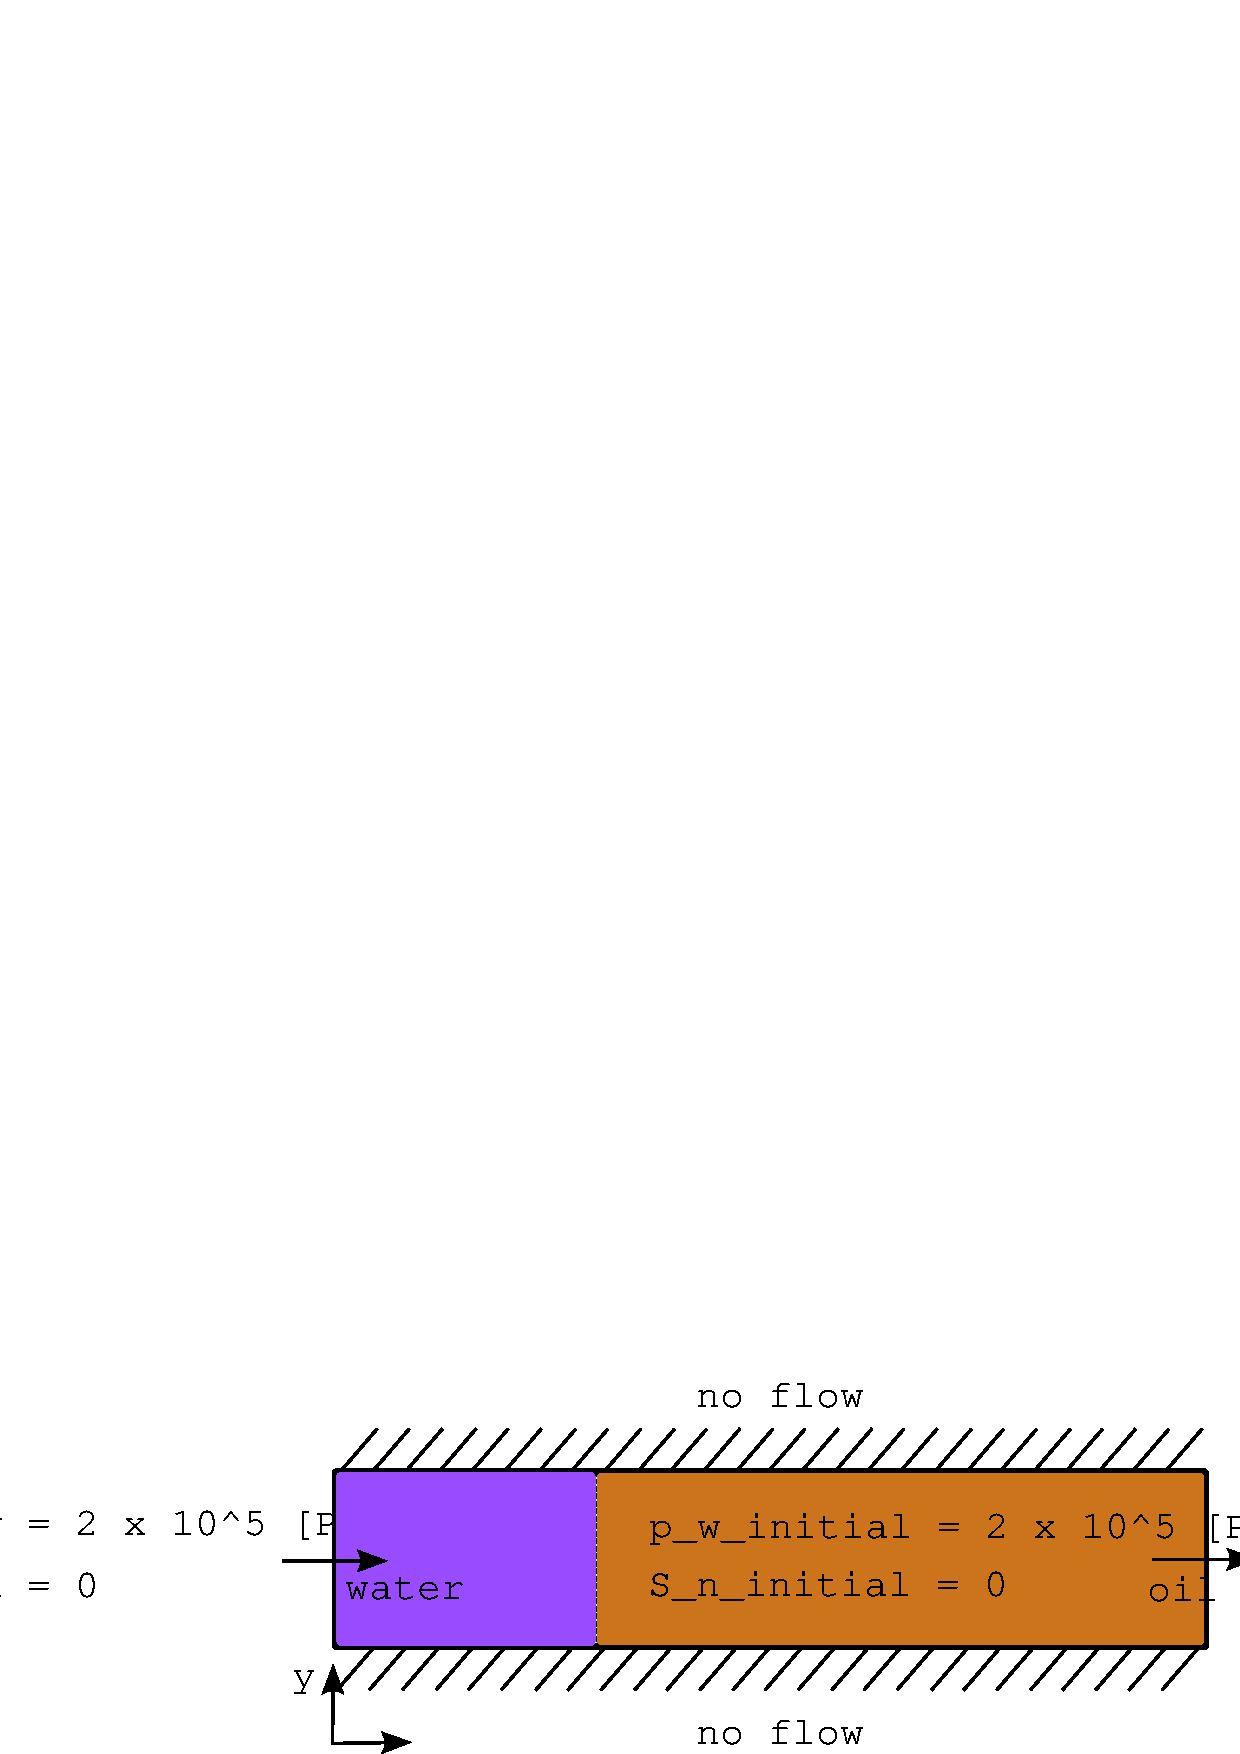
\includegraphics[width=0.9\linewidth,keepaspectratio]{EPS/tutorial-problemconfiguration}
\caption{Geometry of the tutorial problem with initial and boundary conditions.}\label{tutorial-coupled:problemfigure}
\end{figure}

The solved equations are the mass balances of water and oil:
\begin{align}
  \label{massbalancewater}
  \frac {\partial (\phi \, S_{w}\, \varrho_{w})}{\partial t}
  -
  \nabla \cdot \left( \varrho_{w} \, \frac{k_{rw}}{\mu_{w}} \, \mathbf{K}\;\nabla p_w \right)
  -
  q_w
  & =
  0 \\
  \label{massbalanceoil}
  \frac {\partial (\phi \, S_{o}\, \varrho_{o})}{\partial t}
  -
  \nabla \cdot \left( \varrho_{o} \, \frac{k_{ro}}{\mu_{o}} \, \mathbf{K}\;\nabla p_o \right)
  -
  q_o 
  & =
  0
\end{align}

\subsection{The main source file}

Listing \ref{tutorial-coupled:mainfile} shows the main file
\texttt{tutorial/tutorial\_coupled.cc} for the tutorial problem using
a fully-implicit model that assumes immiscibility. This file has to be
compiled and executed in order to solve the problem described above.

\begin{lst}[File tutorial/tutorial\_coupled.cc]\label{tutorial-coupled:mainfile} \mbox{}
  \lstinputlisting[style=eWomsCode, numbersep=5pt, firstline=25, firstnumber=25]{../../tutorial/tutorial_coupled.cc}
\end{lst}

In \eWoms, this file is usually quite short, as most of the work for
setting up the simulation is done by the generic startup routine
\texttt{Ewoms::start()}. The tasks left for the main source file are:
\begin{itemize}
\item Inclusion of the necessary header files from line
  \ref{tutorial-coupled:include-begin} to line
  \ref{tutorial-coupled:include-end}.
\item Specifying the type tag of the problem which is going to be
  simulated at line \ref{tutorial-coupled:set-type-tag}.
\item Starting the simulation using default \eWoms startup routine
  \texttt{Ewoms::start()} on line \ref{tutorial-coupled:call-start}.
\end{itemize}

The default \eWoms startup routine deals with parsing the command line
arguments, reading the parameter file, properly setting up the \Dune
infrastructure, creating the grid, and starting the actual simulation.
Required parameters for the start of the simulation, such as the
initial time-step size, the final simulation time or details of the
grid, can be either specified by command line arguments of the form
(\texttt{--parameter-name=value}), or in the file specified by the
\texttt{--parameter-file="file\_name"} argument. A list of all
parameters that can be specified at run-time can be obtained by passing
the \texttt{--help} argument to the exectutable of the simulation.

\subsection{The problem file}

When solving a problem using \eWoms, the most important file is the
so-called \textit{problem file} as shown in
listing~\ref{tutorial-coupled:problemfile}.

\begin{lst}[File tutorial/tutorialproblem\_coupled.hh]\label{tutorial-coupled:problemfile} \mbox{}
\lstinputlisting[style=eWomsCode, numbersep=5pt, firstline=25, firstnumber=25]{../../tutorial/tutorialproblem_coupled.hh}
\end{lst}

This file specifies everything that is related to the physical
problem. It first sets up the properties relevant for this problem
using the \eWoms property system (for more information see chapter
\ref{sec:propertysystem})
\begin{itemize}
\item First, a new type tag is created for the problem in line
  \ref{tutorial-coupled:create-type-tag}.  In this case, the new type
  tag inherits all properties from the \texttt{BoxImmiscibleTwoPhase}
  type tag, which means that for this problem the immiscible box model
  for two fluid phases is chosen as discretization scheme.
\item On line \ref{tutorial-coupled:set-problem}, the problem class is
  specified for the new type tag, while the kind of grid which is
  going to be used is defined in line \ref{tutorial-coupled:set-grid}
  -- in this case that is \texttt{Dune::YaspGrid}.
\item Since \Dune does not provide a uniform mechanism to initialize
  and load grids, \eWoms features the concept of grid creators. In
  this case, the generic \texttt{CubeGridCreator} is used. This grid
  creator constructs a structured rectangular grid with a specified
  size and resolution. For this grid creator, the physical domain of
  the grid is specified via the run-time parameters
  \texttt{DomainSizeX} and \texttt{DomainSizeY} and its resolution by
  \texttt{CellsX} and \texttt{CellsY}. These parameters can be
  specified via the command-line or in a parameter file, but the
  problem file must define default values for them. Defining these
  defaults is done on lines
  \ref{tutorial-coupled:grid-default-params-begin} to
  \ref{tutorial-coupled:default-params-end}.
\end{itemize}

Next, an appropriate fluid system -- which specifies the thermodynamic
relations of the fluid phases -- has to be chosen. By default, the
fully-implicit immiscible model for two fluid phases uses
\texttt{Ewoms::FluidSystems::TwoPImmiscible}. This fluid system
simplifies things considerably by assuming immiscibility of the
phases, but it requires to explicitly specify the fluids used for the
wetting and non-wetting phases. In this case, liquid water based on
the relations from IAPWS'97~\cite{IAPWS1997} is chosen as the wetting
phase on line \ref{tutorial-coupled:wettingPhase} and liquid oil is
chosen as the non-wetting phase on line
\ref{tutorial-coupled:nonwettingPhase}. The next property, which is
set in line \ref{tutorial-coupled:gravity}, tells the model not to use
gravity. This is then followed by the specifcation default values for
parameters specifying the temporal and spatial domain from line
\ref{tutorial-coupled:default-params-begin} to line
\ref{tutorial-coupled:default-params-end}.  The values of those can be
overwritten at run-time if desired.

Following the property definitions comes the definition of the actual
physical set-up to be simulated. This is done by means of the
\textit{problem class}. The problem class specifies boundary and
initial conditions, source terms or spatial quantities like
temperature, porosity, intrinsic permeability and the parameters of
the material law within the domain. Since there are quite a few
methods of the problem called by the \eWoms models, and often there
are sensible defaults for these methods, it is strongly recomended to
derive the problem class from the class specified by the
\texttt{BaseProblem} property as done on line
\ref{tutorial-coupled:def-problem}\footnote{Technically, deriving the
  problem from the \texttt{BaseProblem} property is not required if it
  implements all necessary methods. Do not complain if things explode
  in this case, though.}.

For isothermal multi-phase porous media model, the problem class must
always provide at least the following methods:
\begin{itemize}
\item \texttt{initial()} for specifying the initial condition within
  the domain,
\item \texttt{source()} which specifies the source term for each conservation quantitym
\item \texttt{boundary()} for specifying the conditions which apply on
  the domain boundary,
\item \texttt{temperature()} specifying the temperature within the
  domain. Note, that if energy is conserved, this method is not
  necessary. Though in this case, energy fluxes must be specified by
  the \texttt{boundary()} and \texttt{source()} methods and an initial
  temperature needs to be defined by the \texttt{initial()} method.
\item \texttt{intrinsicPermeability()} returns the intrinsic
  permeability matrix $\mathbf{K}$ in $[m^2]$ at a given location.
\item \texttt{porosity()} returns the ratio of pore space to
  total volume of the medium at a given location.
\item \texttt{materialLawParams()} returns the function parameters for
  the capillary pressure and relative permeability relations at a
  given location.
\end{itemize}

All of these methods take a single template argument,
\texttt{Context}, and the three function arguments \texttt{context},
\texttt{spaceIdx} and \texttt{timeIdx}. Together, these form the
\textit{execution context}. The execution context can be thought of as
a collection of all available information when a given method is
called. Execution contexts are thus a way to abstract the differences
of the different discretization schemes. The following methods are
provided by all \texttt{context} objects:
\begin{itemize}
\item \texttt{pos(spaceIdx, timeIdx)}: This method returns the
  relevant position of the execution context within the physical
  domain.
\item \texttt{globalSpaceIndex(spaceIdx, timeIdx)}: Returns a global
  index for the spatial entity which is described by the execution
  context. This index can be used to store spatially dependent
  information in an array.
\item \texttt{element()}: Returns the \Dune grid element for which the
  execution context is valid.
\item \texttt{gridView()}: Returns the \Dune grid view of which the
  element is part of.
\item \texttt{problem()}: Returns the \eWoms object which describes
  the physical problem to be solved.
\item \texttt{model()}: Returns the \eWoms model which is used to simulate
  the physical problem.
\end{itemize}

The execution contexts for the \texttt{source} and \texttt{boundary}
methods always provide the following methods in addition:
\begin{itemize}
\item \texttt{volVars(spaceIdx, timeIdx)}: The secondary variables
  used by the model relevant for the execution context. These are
  useful to specify solution dependent source and boundary terms.
\item \texttt{primaryVars(spaceIdx, timeIdx)}: The vector of primary
  variables to which the model solves for.
\end{itemize}

Finally, the execution context for the \texttt{boundary} method
provides the methods \texttt{boundarySegmentArea(spaceIdx, timeIdx)},
and \texttt{normal(spaceIdx, timeIdx)}, which return the area of the
boundary segment and outer unit normal of the boundary segment.

When specifying the boundary conditions in the problem class, a small
safeguard value \texttt{eps\_} should usually be added when comparing
spatial coordinates. For the problem considered here, the left
boundary might not be detected if checking whether the first
coordinate of the global position is equal to zero, but it is detected
reliably by testing whether it is smaller than an
$\epsilon$-value. Also, the \texttt{bboxMax()} (``\textbf{max}imum
coordinate of the grid's \textbf{b}ounding \textbf{box}'') method is
used here to determine the extend of the physical domain. It returns a
vector with the maximum values on each axis of the grid. This method
and the analogous \texttt{bboxMin()} method are provided by the
problem's base class.

In addition to these methods, there might be some additional
model-specific methods. 

\subsection{Defining fluid properties}
\label{tutorial-coupled:description-fluid-class}

The \eWoms distribution includes representations of some common
substances which can be used out of the box. The properties of pure
substances (such as nitrogen, water, or the pseudo-component air) are
provided by header files located in the folder
\texttt{ewoms/material/components}.

When two or more substances are considered, interactions between these
become relevant and the properties of these mixtures of substances --
e.g. composition, density or enthalpy -- are required. In \eWoms, such
interactions are defined by {\em fluid systems}, which are located in
\texttt{ewoms/material/fluidsystems}. A more thorough overview of the
\eWoms fluid framework can be found in
chapter~\ref{sec:fluidframework}.

\subsection{Exercises}
\label{tutorial-coupled:exercises}

The following exercises will give you the opportunity to learn how you
can change soil parameters, boundary conditions, run-time parameters
and fluid properties in \eWoms.

\subsubsection{Exercise 1}

\renewcommand{\labelenumi}{\alph{enumi})}

For Exercise 1 you have to modify the tutorial files only sightly, or
even not at all.

\begin{enumerate}

\item \textbf{Running the Program} \\
  To get an impression what the results should look like, you can first run the original version of 
the fully-implicit tutorial problem by typing  \texttt{./tutorial\_coupled}. 
Note, that the time-step size is automatically adapted during the simulation. 
For visualizing the results using the program \texttt{paraview}, please refer to section \ref{quick-start-guide}.

\item \textbf{Changing the Model Domain} \\
  Change the size of the model domain so that you get a rectangle with
  edge lengths of $\text{x} = \unit[400]{m}$ and $\text{y} =
  \unit[500]{m}$ and with discretization lengths of $\Delta \text{x} =
  \unit[20]{m}$ and $\Delta \text{y} = \unit[20]{m}$. For this, you can
  either change the properties defined between lines
  \ref{tutorial-coupled:default-params-begin} and
  \ref{tutorial-coupled:default-params-end}, or you may pass them as
  command line parameters to the simulation when you run it.

  If you chose to change the problem file, re-compile the simulation
  by typing \texttt{make tutorial\_coupled}.  Note, that you do not
  have to recompile the program if you use command line parameters. In
  both cases, don't forget run the simulation before re-inspecting the
  results using \texttt{paraview}.
  
\item \textbf{Boundary Conditions} \\
  Change the boundary conditions in the problem file
  \texttt{tutorialproblem\_coupled.hh} so that water enters from the
  bottom and oil is extracted from the top boundary. The right and the
  left boundary should be closed for both, water and oil. 

  Note that in \eWoms, flux boundary conditions are specified as
  fluxes of the conserved quantities into the direction of the outer
  normal per area. This means a mass flux into the domain is negative,
  a flux out of the domain is always positive. Re-compile the
  simulation by typing \texttt{make tutorial\_coupled} and re-run it
  as explained above.

\item \textbf{Changing the Shape of the Discrete Elements} \\
  In order to complete this exercise you need a \Dune grid manager
  that is capable of handling simplex grids. By default, \Dune does
  not include such a grid manager in its core modules, but the freely
  available \texttt{ALUGrid}~\cite{ALUGRID-HP} can be used. If you did
  not install such a grid manager, you may also skip this exercise.

  Change the grid creator used by the problem to
  \texttt{SimplexGridCreator<TypeTag>} and the type of the grid to
  \texttt{Dune::ALUSimplexGrid<2, 2>}. The grid creator is specified
  on line \ref{tutorial-coupled:set-gridcreator}, whil the type of the
  \Dune grid manager is set on line
  \ref{tutorial-coupled:set-grid}. You also need to change the include
  statement of the grid creator from \texttt{cubegridcreator.hh} to
  \texttt{simplexgridcreator.hh} on line
  \ref{tutorial-coupled:include-grid-creator} and the one for the grid
  manager from \texttt{dune/grid/yaspgrid.hh} to
  \texttt{dune/grid/alugrid.hh} on line \ref{tutorial-coupled:include-grid-manager}.

  The resulting grid can be examined by re-compiling and starting the
  simulation, loading the result into \texttt{paraview}, and selecting
  \texttt{Surface with Edges} instead of the default visualization
  mode \texttt{Surface}.

\item \textbf{Changing Fluids} \\
  In this exercise you will change the fluids used: Use DNAPL instead
  of LNAPL and Brine instead of Water. This can be done by the
  following steps:
\begin{enumerate}
\item Brine: Brine is thermodynamically very similar to pure water but
  also includes a fixed amount of salt in the liquid phase.  Hence,
  the class \texttt{Ewoms::Brine} calls back to a class which
  represents pure water. (This can be, for example
  \texttt{Ewoms::H2O}, or \texttt{Ewoms::SimpleH2O}.) The class which
  represents pure water is passed to \texttt{Ewoms::Brine} as the
  second template argument after the data type for scalar values,
  i.e. the full definition of the brine component is
  \texttt{Ewoms::Brine<Scalar, Ewoms::H2O<Scalar> >}. The file which
  defines the brine component is located in the folder
  \texttt{ewoms/material/components/}.  Include this file and select
  use the brine component as the wetting phase.
\item DNAPL: Now let us use a component that represents an oil that
  is heavier than water (in environmental engineering this class of
  substances is often called \textbf{d}ense
  \textbf{n}on-\textbf{a}queous \textbf{p}hase \textbf{l}iquid
  (DNAPL)) which is also located in the folder
  \texttt{ewoms/material/components/}. Include the correct file and
  use the DNAPL component as the non-wetting phase.
\end{enumerate}
If you want to take a closer look on how the fluid classes are defined
and which substances are available in the \eWoms distribution, feel
free to browse through the files in the directory
\texttt{ewoms/material/components} and read
chapter~\ref{sec:fluidframework}.

\item \textbf{Use a Full-Fledged Fluid System} \\
  In \eWoms, the canonical way to describe fluid mixtures is via
  \textit{fluid systems}\footnote{For a thorough introduction into
    fluid systems and the concepts related to it, see chapter
    \ref{sec:fluidframework}}.  In order to include a fluid system,
  you first have to comment out lines
  \ref{tutorial-coupled:2p-system-start}
  to \ref{tutorial-coupled:2p-system-end} in the problem file.\\
  Now include the file
  \texttt{ewoms/material/fluidsystems/h2oairfluidsystem.hh}, and
  instruct the model to use this fluid system by setting
  the \texttt{FluidSystem} property via:\\
\begin{lstlisting}[style=eWomsCode]
  SET_TYPE_PROP(TutorialProblemCoupled, 
                FluidSystem,
                Ewoms::FluidSystems::H2OAir<typename GET_PROP_TYPE(TypeTag, Scalar)>)
\end{lstlisting}
However, this is a rather complicated fluid system which considers all
fluid phases as a mixture of the components and also uses tabulated
components that need to be filled with values (i.e. some components
use tables to speed up expensive computations).  The initialization of
the fluid system is normally done in the constructor of the problem by
calling \texttt{FluidSystem::init();}.

As water flow replacing a gas is much faster, simulate the problem
only until $2.000$ seconds is reached and start with a time step of
$1$ second.

Now, revert the changes made in this part of the exercise, as we will
continue to use immiscible phases from here on and hence do not need a
complex fluid system.

\item \textbf{Changing Constitutive Relations} \\
  Instead of using a regularized Brooks-Corey law for the relative
  permeability and for the capillary pressure saturation relationship,
  use an linear material law which does not consider residual
  saturation. The new material law should exhibit an entry pressure of
  $p_e = 0.0\;\text{Pa}$ and maximal capillary pressure of
  $p_{c_{max}} = 2000.0\;\text{Pa}$. To do that, you have to change
  the material law property on line
  \ref{tutorial-coupled:eff2abs} as follows:
\begin{itemize}
\item First, switch to the linear material law. This can be achieved
  by replacing \texttt{RegularizedBrooksCorey} in the private section
  of the property definition by \texttt{LinearMaterial} and rename
  \texttt{RawMaterialLaw} to \texttt{TwoPMaterialLaw}. Also remove the
  line which contains the \texttt{EffToAbsLaw} typedef.
\item Then, adapt the necessary parameters of the linear law and the
  respective \texttt{set}-functions can be found in the file
  \texttt{ewoms/material/fluidmatrixinteractions/2p/linearmaterialparams.hh}.\\
  Call the \texttt{set}-functions from the constructor of the problem.
\item Finally, re-compile and re-run the simulation. In order to
  successfully compile the simulation, you also have to include the
  header file which contains the linear material law. This header is
  called \texttt{linearmaterial.hh} and is located in the same
  directory as the header for the regularized Brooks-Corey law,
  \texttt{regularizedbrookscorey.hh}.
\end{itemize}
 
\item \textbf{Heterogeneities}  \\
  Set up a model domain with the soil properties given in Figure
  \ref{tutorial-coupled:exercise1_d}. Adjust the boundary conditions
  so that water is flowing from the left to the right of the domain again.
\begin{figure}[ht]
\psfrag{K1 =}{$\mathbf{K} = 10^{-8}\;\text{m}^2$}
\psfrag{phi1 =}{$\phi = 0.15$}
\psfrag{K2 =}{\textcolor{white}{$\mathbf{K} = 10^{-9}\;\text{m}^2$}}
\psfrag{phi2 =}{\textcolor{white}{$\phi = 0.3$}}
\psfrag{600 m}{$600 \;\text{m}$}
\psfrag{300 m}{$300 \;\text{m}$}
\centering
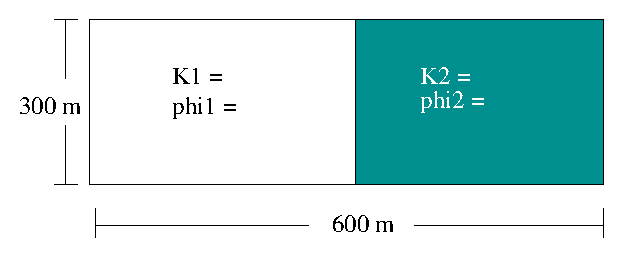
\includegraphics[width=0.5\linewidth,keepaspectratio]{EPS/exercise1_c.eps}
\caption{Exercise 1f: Set-up of a model domain with a heterogeneity. $\Delta x = 20 \;\text{m}$ $\Delta y = 20\;\text{m}$.}\label{tutorial-coupled:exercise1_d}
\end{figure}
You can use the fluids of exercise 1b).

\textbf{Hint:} The relevant position in the domain can be obtained using
\texttt{const auto \&pos=context.pos(spaceIdx, timeIdx);}

When does the front cross the material border? In paraview, the
animation view (\textit{View} $\rightarrow$ \textit{Animation View})
is a convenient way to get a rough feeling of the time-step sizes.
\end{enumerate}

\subsubsection{Exercise 2}

For this exercise, first create a new problem file analogous to the
file \texttt{tutorialproblem\_coupled.hh} (e.g. with the name
\texttt{ex2\_tutorialproblem\_coupled.hh} and new spatial parameters
just like \texttt{tutorialspatialparams\_coupled.hh}. The new problem
file needs to be included in the file \texttt{tutorial\_coupled.cc}.

The new file should contain definitions of new classes with names that
relate to the file name, such as
\texttt{Ex2TutorialProblemCoupled}. Make sure that you also adjust the
guardian macros in lines \ref{tutorial-coupled:guardian1} and
\ref{tutorial-coupled:guardian1} in the header files (e.g. change
\mbox{\texttt{EWOMS\_TUTORIALPROBLEM\_COUPLED\_HH}} to
\mbox{\texttt{EWOMS\_EX2\_TUTORIALPROBLEM\_COUPLED\_HH}}). Include the
new problem file in \texttt{tutorial\_coupled.cc}.  Besides adjusting
the guardian macros, the new problem file should define and use a new
type tag for the problem as well as a new problem class
e.g. \mbox{\texttt{Ex2TutorialProblemCoupled}}. The type tag for the
problem should be adjusted, too. For this, modify line
\ref{tutorial-coupled:set-type-tag} in the problem file and the adapt
the \texttt{main} function in the file \texttt{tutorial\_coupled.cc}.

After this, change the domain parameters so that they match the domain
described by figure \ref{tutorial-coupled:ex2_Domain}. Adapt the
problem class so that the boundary conditions are consistent with
figure \ref{tutorial-coupled:ex2_BC}. Initially, the domain is fully
saturated with water and the pressure is $p_w = 5\cdot
10^5\;\text{Pa}$. Oil infiltrates from the left side. Create a grid
with $20$ cells in $x$-direction and $10$ cells in $y$-direction. The
simulation time should end at $10^6\;\text{s}$ with an initial time
step size of $100\;\text{s}$.

\begin{figure}[ht]
\psfrag{K1}{K $= 10^{-7}\;\text{m}^2$}
\psfrag{phi1}{$\phi = 0.2$}
\psfrag{Lin}{\textsc{Brooks}-\textsc{Corey} Law}
\psfrag{Lin2}{$\lambda = 1.8$, $p_e = 1000\;\text{Pa}$}
\psfrag{K2}{K $= 10^{-9}\;\text{m}^2$}
\psfrag{phi2}{$\phi = 0.15$}
\psfrag{BC1}{\textsc{Brooks}-\textsc{Corey} Law} 
\psfrag{BC2}{$\lambda = 2$, $p_e = 1500\;\text{Pa}$}
\psfrag{H1y}{$50\;\text{m}$}
\psfrag{H2y}{$15\;\text{m}$}
\psfrag{H3y}{$20\;\text{m}$}
\psfrag{L1x}{$100\;\text{m}$}
\psfrag{L2x}{$50\;\text{m}$}
\psfrag{L3x}{$25\;\text{m}$}
\centering
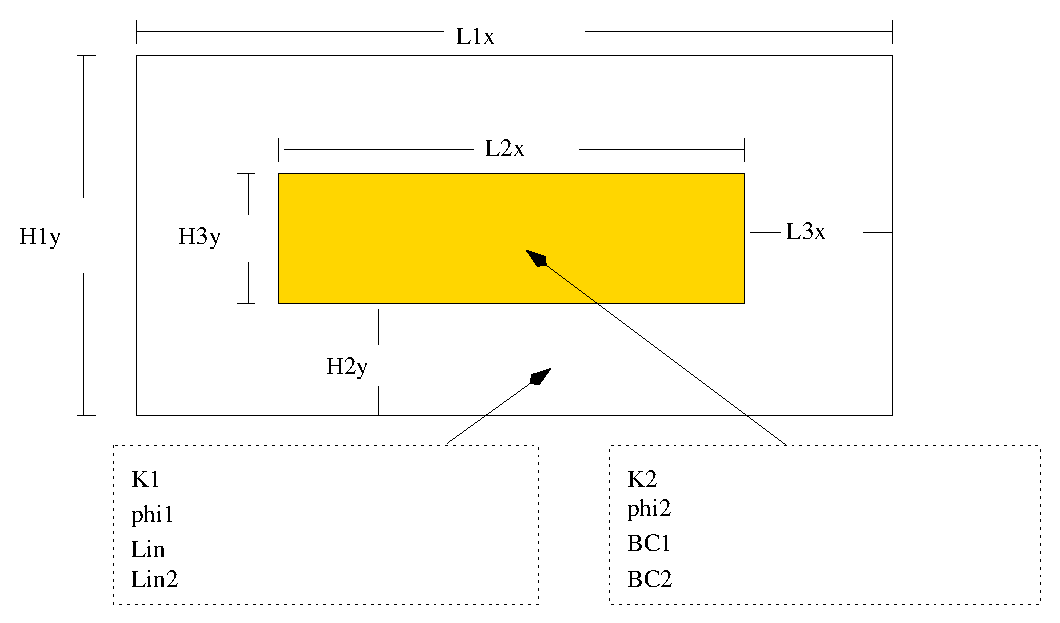
\includegraphics[width=0.8\linewidth,keepaspectratio]{EPS/Ex2_Domain.eps}
\caption{Set-up of the model domain and the soil parameters}\label{tutorial-coupled:ex2_Domain}
\end{figure}

\begin{figure}[ht]
\psfrag{pw}{$p_w = 5 \times 10^5\;\text{Pa}$}
\psfrag{S}{$S_n = 1.0$}
\psfrag{qw}{$q_w = 2 \times 10^{-4} \;\text{kg}/\text{m}^2\text{s}$}
\psfrag{qo}{$q_n = 0.0 \;\text{kg}/\text{m}^2\text{s}$}
\psfrag{no flow}{no flow}
\centering
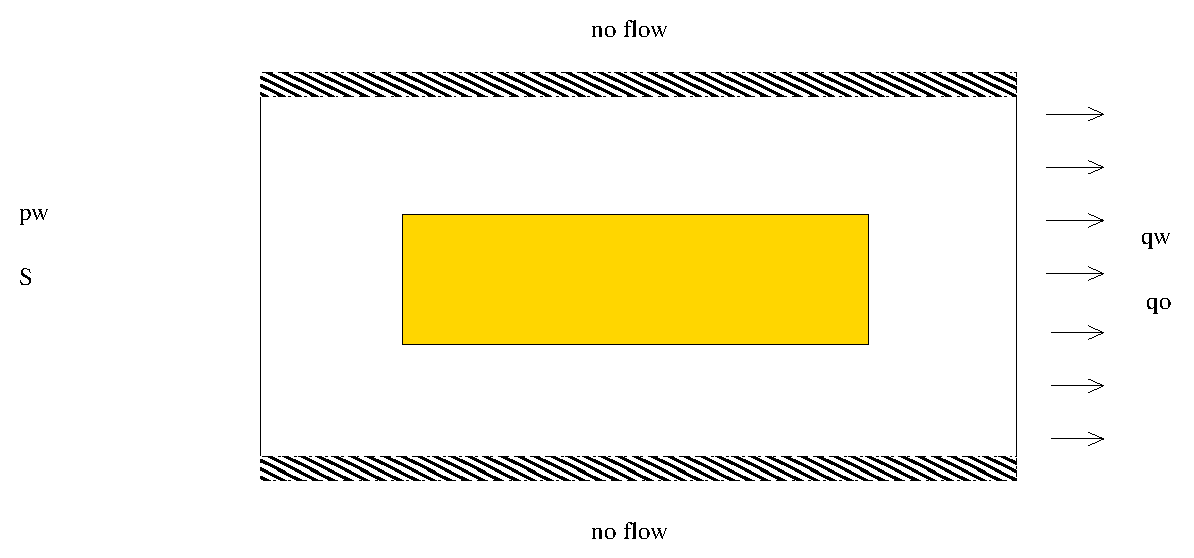
\includegraphics[width=0.8\linewidth,keepaspectratio]{EPS/Ex2_Boundary.eps}
\caption{Boundary Conditions}\label{tutorial-coupled:ex2_BC}
\end{figure}

\begin{itemize}
\item Increase the simulation time to e.g. $4\times 10^7
  \;\text{s}$. Investigate the saturation of the wetting phas: Is the
  value range reasonable?
\item What happens if you use a grid with more cells in each direction?
\end{itemize}

\subsubsection{Exercise 3: Create a New Component}

Create a new file for the benzene component called \texttt{benzene.hh}
and implement a new component. (\textbf{Hint:} The easiest way to do
this is to copy and modify one of the existing components located in
the directory \texttt{ewoms/material/components}.) Use benzene as a
new non-wetting fluid and run the problem of Exercise 2 with water and
benzene. Benzene has a density of $889.51 \, \text{kg} / \text{m}^3$
and a viscosity of $0.00112 \, \text{Pa} \; \text{s}$.

\clearpage \newpage

%%% Local Variables: 
%%% mode: latex
%%% TeX-master: "ewoms-handbook"
%%% End: 
